\documentclass[twocolumn]{aastex631}

% Packages you've added in

\usepackage{booktabs}
\usepackage{graphicx}


\newcommand{\vdag}{(v)^\dagger}
\newcommand\aastex{AAS\TeX}
\newcommand\latex{La\TeX}
\newcommand{\code}[1]{\texttt{#1}}



\begin{document}

    \title{High Resolution Cross-Correlation Transmission Spectroscopy of KELT-20b/MASCARA-2b: Phase-resolved Line Velocities and Asymmetries} \footnote{Based on data acquired with the Potsdam Echelle Polarimetric and Spectroscopic Instrument (PEPSI) using the Large Binocular Telescope (LBT) in Arizona.}

    \author[0009-0001-1459-3738]{Calder Lenhart}
    \affiliation{Department of Astronomy, The Ohio State University \\ 4055 McPherson Laboratory, 140 West 18th Avenue \\ Columbus, OH 43210}

    \author[0000-0002-5099-8185]{Marshall C. Johnson}
    \affiliation{Department of Astronomy, The Ohio State University \\ 4055 McPherson Laboratory, 140 West 18th Avenue \\ Columbus, OH 43210}
    
    \author[0000-0002-4361-8885]{Ji Wang(王吉)}
    \affiliation{Department of Astronomy, The Ohio State University \\ 4055 McPherson Laboratory, 140 West 18th Avenue \\ Columbus, OH 43210}
    
    \author[0000-0002-8823-8237]{Anusha Pai Asnodkar}
    \affiliation{Department of Astronomy, The Ohio State University \\ 4055 McPherson Laboratory, 140 West 18th Avenue \\ Columbus, OH 43210}

    \author{Sydney Petz}
    \affiliation{Department of Astronomy, The Ohio State University \\ 4055 McPherson Laboratory, 140 West 18th Avenue \\ Columbus, OH 43210}

    \author[0000-0002-6192-6494]{Klaus Stassmeier}
    \affiliation{Leibniz-Institut für Astrophysik Potsdam, An der Sternwarte 16 D-14482 Potsdam, Germany}

    \author[0000-0002-0551-046X]{Ilya Ilyin}
    \affiliation{Leibniz-Institut für Astrophysik Potsdam, An der Sternwarte 16 D-14482 Potsdam, Germany}


    \begin{abstract}
        We present high-resolution cross-correlation transmission spectroscopy results from a lone observation of KELT-20b with the PEPSI spectrograph on the LBT. We detect Fe I, Fe II, Mg I, Na I, and Cr I and tentatively detect Ba II, Cu I, and Mn I among an inventory of 59 atoms, ions, and molecules. We phase-resolve the Doppler shifts of each detected species and bin both ingress/egress and first/second half CCFs to highlight limb asymmetries and longitudinal variations in the atmosphere's wind structure, finding several high-confidence species redshifting with phase which serves to challenge current theory. We detail the potential drivers of observed phase asymmetries, providing evidence for several dynamical, chemical, and radiative mechanisms in KELT-20b by connecting our observation to general circulation models. We note the continued absence of molecular thermal inversion agents, with further support for atomic Fe I and Fe II as the low pressure absorbers. Due to KELT-20b's ionosphere, we probe vertical wind structures with phase-dependent velocity offsets between the lower-pressure Fe II ($15.5\sigma$) and deeper Fe I ($5.3\sigma$). We attempt to constrain the planet's magnetic field via the moderately heavy ion Ba II.

        
    \end{abstract}

    \keywords{Doppler shift, Exoplanet atmospheric dynamics, Exoplanet atmospheric structure, High resolution spectroscopy, Hot Jupiters, Transmission spectroscopy}


    \section{Introduction}\label{sec:intro}

        Ultra hot Jupiters (UHJs) represent an exceptional subclass of exoplanets, particularly amenable to atmospheric characterization. These planets have highly irradiated, often tidally locked atmospheres, with dayside temperatures exceeding 2200K. On the intensely hot dayside, molecular constituents dissociate into atomic and ionic species. These species are transported across the terminator—--marked by a significant day-night temperature contrast—--to the cooler nightside through various dynamical processes. The gaseous, puffy atmospheres of UHJs provide a unique environment to study chemical, radiative, and dynamical energy transport processes and their interactions. This study focuses on the dynamics, a crucial component of the energy budget in UHJ atmospheres.


        KELT-20b/MASCARA-2b is positioned among the ultra hot Jupiter regime for extreme dynamics favorably, with wind speeds up to $\sim5\,kms^{-1}$ \citep{Tan2019}, with an orbital period of $3.474\,\text{d}$, radius of $1.741\,R_{J}$, dayside temperature ($T_{eq}$) of $2262K$, and a bright ($m_V\sim7.6$) A2V host star, HD 185603 \citep{Lund2017}. It has been observed with the CARMENES \citep{CasasayasBarris2019, Nugroho2020, Kesseli2020}, EXPRES \citep{Hoeijmakers2020}, FIES \citep{BelloArufe2022}, and HARPS-N \citep{CasasayasBarris2019, Rainer2021, Langeveld2022, Sicilia2022} spectrographs previously. These observations have produced detections of Fe I, Fe II, Na I, Ca II, and tentative detections of Mg I and Cr II.

        Transmission spectroscopy is the foremost method for probing the upper atmospheres of exoplanets, allowing us to explore the most extreme pressure regimes on UHJs. In these regions, day-night winds and equatorial jets redistribute heat to the nightside.
        
        
        
        
        Previously, measuring UHJ wind speeds using transmission spectroscopy exclusively involved stacking the cross-correlation functions (CCFs) from the entire transit's spectra. This approach maximizes the signal-to-noise ratio (SNR) but sacrifices phase-dependent analysis, thus limiting our understanding of three-dimensional wind structures \citep{MillerRicciKempton2012}. The advent of ground-based spectrographs with resolutions of $R\sim10^{5}$  has enabled phase-resolved high-resolution cross-correlation transmission spectroscopy (HRCCTS) studies. These studies have yielded comprehensive profiles of atmospheric constituents and their asymmetrical velocity fields. By binning CCFs between ingress/egress and first/second half of the transit and observing their relative velocity offsets, we can map a range of dynamical, radiative, chemical mechanisms \citet{Savel2023}. Phase-resolved Doppler-shifted cross-correlation signals of (nominally) individual species templates and high resolution transmission spectra are one of the most promising tools in exoplanetary characterization, granting an unprecedented opportunity for interface between atmospheric theory and observation.

        
            
        There are at least five limitations inherent to the cross-correlation technique, three of which we account for in this paper: (1) An often overlooked assumption in HRCCTS is that one template (the model spectrum) species' absorption lines does not overlap one or more other templates, thus assuming each CCF's significance only corresponds to the search species---also known as aliasing. Aliasing between the absorption lines of a search species (the data) and a different species template can alter true absorption signals and create spurious signals. We present methodology for and results of aliasing checks between template species, and confirm each of our reported detections have no significant aliasing components modifying their signal. (2) Measuring KELT-20's systemic velocity from its stellar lines is not straightforward. \citep{Pino2022} (3) We are limited to a single observation with PEPSI, losing out on nondetected species' absorption lines and potentially reducing recovered species' CCF amplitudes (see Figure \ref{fig:model-spectra-appendix}). Recently, studies of UHJs have combined observations from multiple spectrographs. In the case of KELT-20b, there are two studies using observations from more than one spectrograph, \citet{CasasayasBarris2019} and \citet{Nugroho2020}, but these are not combined. (4) Line lists


        Phase-resolved velocity offsets of UHJs have been analyzed for WASP-19b \citep{}, WASP-33b \citep{Cauley2021}, WASP-76b \citep{Ehrenreich2020, Kesseli2022}, WASP-121b \citep{Wardenier2024}, WASP-189b \citep{Prinoth2023}, KELT-9b \citep{Cauley2019, Pino2022}, and KELT-20b \citep{Hoeijmakers2020, Rainer2021}. Consistent with GCMs \citep{},  


        This work seeks to reproduce previous detections of atomic species in KELT-20b's atmosphere, make novel detections, and phase-resolve the Doppler-shifted signals of each species over the course of transit to observe distinct longitudinal slices and pressure regimes. With greater resolving power comes the responsibility of disentangling the imprints of numerous three-dimensional physical mechanisms in the phase-resolved CCFs. When equipped with signals that maintain, at minimum, an SNR exceeding $3\sigma$ over the course of transit, we intend to diagnose drivers of phase asymmetries by relating a suite of phase-resolved CCFs of each species to GCM results.

        Ultra hot Jupiter magnetic 
        Using heavy ion velocity offsets, we will also attempt to constrain KELT-20b's magnetic field \citep{Savel2024}.

      

        With a lone observation of KELT-20b's transit using the PEPSI spectrograph on the LBT, we confirm detections of Mg I, Fe I, Fe II, and Na I and present novel species Cr I, Ba II, Cu I, and Mn I, each complete with several modes of phase-binning to highlight limb asymmetries. We do not reproduce detections of H I, Ca II, Cr II, and FeH. Additionally, we provide a compendium of results from HRCCTS studies of KELT-20b to review the consensus of KELT-20b's atmospheric constituents and dynamical features. We highlight the relative velocity offsets and ingress/egress asymmetries of our strongest detections, Mg I ($5.4\sigma$), Fe I ($5.3\sigma$), and Fe II ($15.5\sigma$), offering a view of wind velocities in several pressure regimes and constraints on day-night flows. We also detail the phase-resolved velocity of Ba II ($3.3\sigma$), a moderately heavy ion that, with respect to neutral ion velocities, can constrain the behavior of KELT-20b's magnetic field \citep{Savel2024}. 

        This paper describes characteristics of the transit observation in Section \ref{sec:Observations}. In Section \ref{sec:Methodology}, Methodology, we describe the generation of model spectra and data processing of observed spectra, data cleaning steps, cross-correlation of the two, and the methods to produce phase-resolved data. In Section \ref{sec:Results}, Results, we compile detections from all previous high-resolution transmission spectroscopy and HRCCTS papers alongside our own, along with phase-resolved velocity offsets and discussion of nondetections and aliasing. In Conclusions, Section \ref{sec:Conclusions}, we discuss the implications our results have for future observations and theory. Finally, we present plots of the generated transmission spectra in Section \ref{app:Model transmission spectra}, 1D CCFs and 2D CCFs of detected species in Section \ref{app:Detections}, phase-binned velocity offsets in Section \ref{app:Dynamics}, 1D CCFs and 2D CCFs of salient nondetections in Section \ref{app:Nondetections}, and aliases with Fe I and Fe II in Section \ref{app:Aliases}.
        
    \section{Observations}\label{sec:Observations}
        We obtained our data with the ${\mathcal{R} = 130000}$ Potsdam Echelle Polarimetric and Spectroscopic Instrument (PEPSI)\citep{Strassmeier2015} on the Large Binocular Telescope (LBT). We utilized the PEPSI CD III+V bandpass, with a red arm wavelength coverage of 4800--5441\AA\ and blue arm of 6278--7419\AA\. To maximize signal recovery without losing precision in velocity offsets due to Doppler smearing\footnote{Doppler smearing occurs when the planetary radial velocity changes more than a resolution element during an exposure. At mid-transit, the maximum exposure time of PEPSI that avoids Doppler smearing of the atmospheric signal of KELT-20b is $\Delta t \sim \frac{cP}{2\pi \mathcal{R} K_p} \sim 650~\text{s}$, where $c$ is the speed of light, $P$ is the period of the planet, $\mathcal{R}$ is the resolution of the spectrograph, and $K_p$ is the planetary radial velocity semi-amplitude (see Equation \ref{equ:RV_p})\citep{Wardenier2024, BoldtChristmas2024}.}, we took $600~\text{s}$ exposures. We list the remaining key observation parameters in Table~\ref{tab:observation_details}. We reduced this observation using the Spectroscopic Data Systems (SDS) Pipeline. 

        \begin{deluxetable}{lc}
            \tablecaption{Observation details for 2019 May 4 transit.\label{tab:observation_details}}
            \tablehead{
                \colhead{\textbf{Parameter}} & \colhead{\textbf{Value}}
            }
            \startdata
            Telescope & LBT \\
            Instrument & PEPSI \\
            $N_{\text{obs}}$ & 23 \\
            $N_{\text{obs, in-transit}}$ & 21 \\
            $T_{exp}$ (s) & 600 \\
            Airmass Range & 1.00--2.01 \\
            Phases Covered & $-0.023$--0.034 \\
            $S/N_{\text{blue}}$ & 288 \\
            $S/N_{\text{red}}$ & 308 \\
            \enddata
        \end{deluxetable}

        \begin{figure}
            \centering
            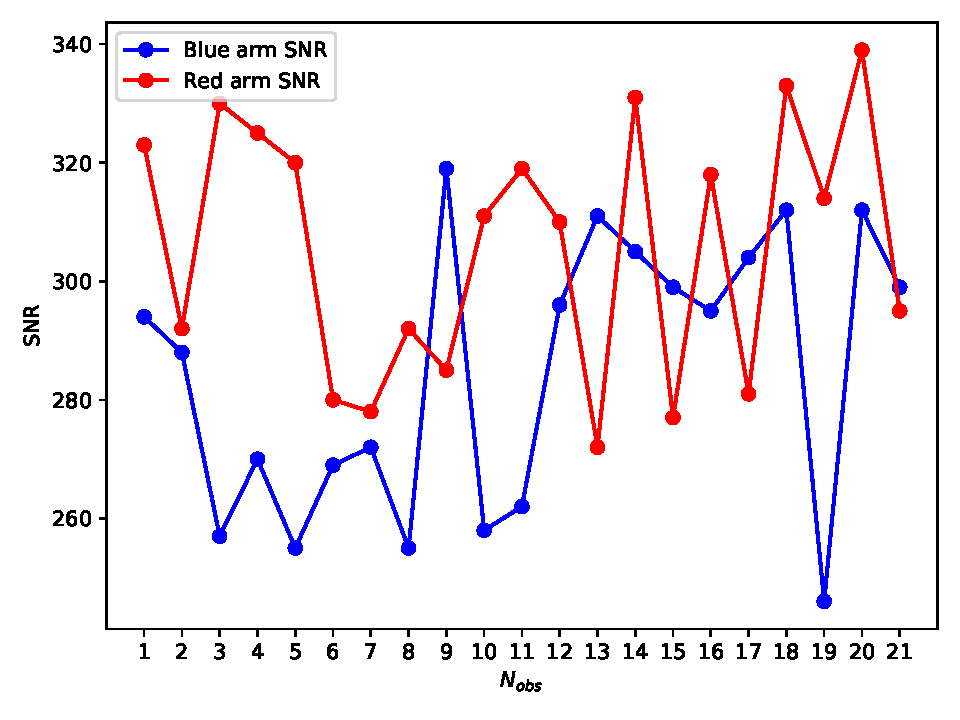
\includegraphics[width=0.5\textwidth]{plots/SNR.pdf}
            \caption{SNR vs exposure, showing a relatively consistent observation quality over the course of transit. Note that the early and late observations, corresponding to transit ingress and egress, have a SNR $\sim300$}.
            \label{fig:SNR}
        \end{figure}
        
    
    \section{Methodology}\label{sec:Methodology}

        \subsection{Model Spectra}\label{subsec:Model Spectra}
            We generate model transmission spectra, in 0.01\AA\ steps from 3850--7500\AA, with the \code{petitRADTRANS} package~\citep{petitRADTRANS}, as shown in Figure~\ref{fig:main-spectra}. These spectra cover the PEPSI CD III+V bandpass. We assume stellar and planetary parameters from~\citet{Lund2017}, listed in Table~\ref{tab:parameters_summary}. We select a P-T profile given by Equation (29) of~\citet{Guillot2010} with best-fit parameters $\gamma = 30$ and $K_{IR} = 0.04$ as obtained in a grid search in~\citet{Johnson2023}. While these parameters were derived using emission spectra, transmission spectra are less sensitive to detailed vertical temperature structures~\citep{Kesseli2020}. Since our analysis concerns the atmosphere's dynamics as opposed to chemistry, we deem the same profile sufficient for this analysis. 
            We calculate volume mixing ratios (VMRs) for each species using the \code{PyFastChem} equilibrium chemistry model~\citep{Stock2018, Stock2022, Kitzmann2023}, assuming solar abundances~\citep{Asplund2021} and the aforementioned P-T profile. We assume that quenching, a mechanism by which atmospheric abundances diverge from those predicted by chemical equilibrium at a certain pressure, occurs at 1 bar. Thus, we approximate each species' VMR as equal to its maximum VMR at 1 bar, calculated by \code{PyFastChem}~\citep{Johnson2023,Petz2023}. We also set the VMRs of ionized species equal to those of their neutral counterparts to simplify our analysis. 
            Atomic and molecular opacities were sourced from the~\code{petitRADTRANS} database, with missing entries supplemented from the DACE Opacity Database\footnote{\url{https://dace.unige.ch/opacityDatabase/}}, converted to \code{petitRADTRANS}-compatible format (P. Mollière, private communication). \code{peitRADTRANS} sources its atomic opacities from the Kurucz line list, and we ensured the DACE opacities---Na I and Co I---came from the same line list.~\footnote{\url{http://kurucz.harvard.edu/}}. We used several DACE molecular opacity datasets, including the ATP line list for AlO \citep{ATP}, VBATHY line list for CaO \citep{VBATHY}, and Rivlin line list for NaH \citep{Rivlin}.
            
            \begin{deluxetable*}{l l c c}\label{tab:parameters_summary}
                \tablecaption{This table summarizes the planetary and stellar parameters relevant to our analysis. Sources: a:~\citet{Lund2017}; b:~\citet{Johnson2023}.}
                \tablehead{
                    \colhead{\textbf{Description}} & \colhead{\textbf{Parameter}} & \colhead{\textbf{Value}} & \colhead{\textbf{Source}}
                }
                \startdata
                    \multicolumn{4}{c}{\textbf{Planetary Parameters}} \\
                    \midrule
                    Planet Radius & $R_P$ ($R_{\oplus}$) & 19.51 &a\\
                    Planet Mass & $M_P$ ($M_{\oplus}$) & 1072 &a\\
                    Equilibrium Temperature & $T_{\text{eq}}$ (K) & 2262 &a\\
                    Orbital Period & $P$ (d) & 3.4741085 &a\\
                    Epoch of Mid-Transit & $T_0$ (BJD\_TDB) & 2457485.74965 &a\\
                    Planetary Radial Velocity Semi-amplitude & $K_{p,expected}$ (km s$^{-1}$) & $169 \pm 6$ &a\\
                    Systemic Velocity & $v_{\text{sys}}$ (km s$^{-1}$) & $-26.0$ &b\\
                    Projected Equatorial Rotational Velocity & $v \sin i_P$ (km s$^{-1}$) & 2.5 &a\\
                    Infrared Opacity & $\kappa_{\text{IR}}$ & 0.04 &b\\
                    Ratio of Optical to Infrared Opacities & $\gamma$ & 30 &b\\
                    Reference Pressure & $P_0$ (bar) &a&b\\
                    Atmospheric Abundance of H & $X_{\text{H}_2}$ & 0.7496 &b\\
                    Atmospheric Abundance of He & $X_{\text{He}}$ & 0.2504 &b\\
                    Volume Mixing Ratio of H$^-$ & VMR (H$^-$) & $1 \times 10^{-9}$ &b\\
                    \midrule
                    \multicolumn{4}{c}{\textbf{Stellar Parameters}} \\
                    \midrule
                    Stellar Radius & $R_{\ast}$ ($R_{\sun}$) & 1.565 &a\\
                    Stellar Mass & $M_{\ast}$ ($M_{\sun}$) & 1.76 &a\\
                    Stellar Effective Temperature & $T_{\text{eff}}$ (K) & 8720 &a\\
                    Metallicity & $[$Fe/H$]$ & $-0.29$ &a\\
                                & $v_{sys}$ (km s$^{-1}$) & -26.0 & b\\
                \enddata
            \end{deluxetable*}

            We calculated an observability score for each neutral atomic species we searched for. In addition, we searched for
            \begin{figure}
                \centering
                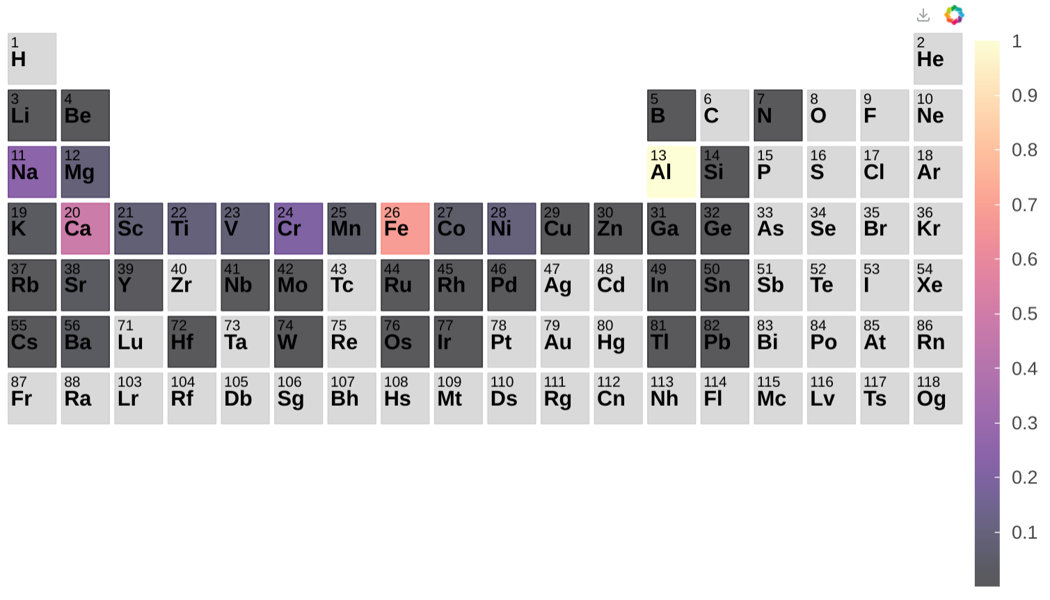
\includegraphics[width=0.5\textwidth]{observability_scores.png}
                \caption{Observability scores for each species were calculated using a modified version of the methodology from \citet{Kesseli2022}. The score \(S_i\) for species \(i\) is determined by the following equation:
                \begin{equation}
                S_i = \frac{1}{\max(S)} \left[ \int_{\lambda_\text{min, red}}^{\lambda_\text{max, red}} \left( \ln \tau_\text{all}(\lambda) - \ln \tau_i(\lambda) \right) \, d\lambda + \int_{\lambda_\text{min, blue}}^{\lambda_\text{max, blue}} \left( \ln \tau_\text{all}(\lambda) - \ln \tau_i(\lambda) \right) \, d\lambda \right]
                \end{equation}
                Here, \(\lambda_\text{min, red}\) and \(\lambda_\text{max, red}\) are the minimum and maximum wavelengths for the PEPSI red arm, respectively, and \(\lambda_\text{min, blue}\) and \(\lambda_\text{max, blue}\) are the corresponding wavelengths for the blue arm. \(\tau_\text{all}\) represents the total opacity across all species, while \(\tau_i\) is the opacity excluding the species of interest. \(\max(S)\) denotes the maximum value of the unnormalized scores.}
            \end{figure}

            
            
        \subsection{Data Preparation}\label{subsec:Data Preparation}
            The following procedure is nearly identical to that of \citet{Johnson2023} and \citet{Petz2023}. First, we import the flux values for each spectrum recorded, then regrid the fluxes to common wavelength values for each spectrum. Next, we flatten both arms of the time-series spectra by subtracting off the median flux from each, yielding residual spectra with stellar lines and time-invariant telluric lines removed. Next, we remove systematics from the spectra. Our systematics correction method is unique in that tit employs both the~\code{molecfit} package~\citep{Smette2015, Kausch2015} and a modified version of the \code{PySysRem}~\footnote{https://github.com/stephtdouglas/PySysRem} package that accepts PEPSI data.~\code{molecfit} fits a model of the telluric spectrum to the data, finds the best-fit model, then removes it. The SYSREM detrending algorithm~\citep{Tamuz2005} fits and removes systematic effects, with the number of systematics to correct for ($N_{\mathrm{Sys}}$) and the number of SYSREM iterations ($N_{\mathrm{Iter}}$) being the relevant input parameters. As determined in~\citet{Johnson2023}, applying both methods yields increased significance of retrieved signals than either alone. We first use~\code{molecfit} to fit and remove telluric lines in the red arm spectra only, as the blue arm is absent of significant tellurics~\citep{Smette2015}. Finally, we apply SYSREM to the residual spectra, empirically determining the number of iterations to apply to the spectra, the amount which yields the greatest recovered SNR in each species, as shown in Table~\ref{tab:sysrem_and_vmr}.
 

        \begin{deluxetable*}{lcccc}
            \tablecaption{Optimal SYSREM iterations, $N_{\mathrm{Sys}}$, for systematics reduction for each species meeting the tentative detection. We bin the telluric and non-telluric contaminated wavelength regions, finding the best $N_{\mathrm{Sys}}$ for each. Note that the blue arm does not contain any tellurics, so it only contains one $N_{\mathrm{Sys}}$ parameter for non-telluric regions.}
            \label{tab:sysrem-and-vmrs}
            \tablehead{
                \colhead{\textbf{Species}} & 
                \colhead{$\textbf{N}_{\mathrm{Sys},\text{Red}}$ (Non-telluric)} & 
                \colhead{$\textbf{N}_{\mathrm{Sys},\text{Red}}$ (Telluric)} & 
                \colhead{$\textbf{N}_{\mathrm{Sys},\text{Blue}}$} & 
                \colhead{VMR}
            }
            \startdata
            Mg I & 1 & 1 & 3 & $6.08 \times 10^{-5}$ \\
            Fe I & 5 & 5 & 6 & $4.95 \times 10^{-5}$ \\ 
            Fe II & 5 & 5 & 5 & $4.95 \times 10^{-5}$ \\
            Na I & 0 & 10 & 2 & $2.82 \times 10^{-6}$ \\
            Cr I & 1 & 1 & 3 & $7.08 \times 10^{-7}$ \\
            Cr II & 1 & 1 & 3 & $7.08 \times 10^{-7}$ \\
            Co I & 0 & 10 & 5 & $1.49 \times 10^{-7}$ \\
            Zn I & 1 & 1 & 3 & $6.23 \times 10^{-8}$ \\
            Ca I & 0 & 10 & 5 & $2.10 \times 10^{-8}$ \\
            Cu I & 1 & 1 & 3 & $2.06 \times 10^{-8}$ \\
            Ti II & 1 & 1 & 3 & $5.63 \times 10^{-9}$ \\
            \enddata
        \end{deluxetable*}
    
        \subsection{Cross-correlation}\label{subsec:cross-correlation}
            With data preparation complete, we cross-correlate model and observed spectra in the stellar rest frame, with the same procedure as described in~\citet{Johnson2023}. The cross correlation function is defined as
            \begin{equation} \label{equ:CCF}
                \text{CCF}(v,t) = \sum_{i}\frac{f_iT_i}{\sigma_i^{2}} 
            \end{equation} 
            where $f_i$ is the observed flux, $T_i$ is the Doppler shifted template spectrum, and $\sigma_i^2$ is the variance of the flux. The cross-correlation procedure is adapted from the BANZAI-NRES package~\citep{McCully2022}. Per-spectrum SNR is defined as
            \begin{equation} \label{equ:SNR}
                \text{SNR}_i = P_{90}\left(\frac{f_i}{\sigma_i}\right)
            \end{equation}
            where we take the 90th percentile of the ratio of flux to error for the i\textsuperscript{th} spectrum. Per-spectrum CCF weights are found by computing
            \begin{equation}\label{equ:CCF_weight}
                    \text{CCF}_{\text{weight}, i} = \text{SNR}_i  \cdot \sum [ \max(T_i) - T_i ]
            \end{equation}
            where $\sum [ \max(T_i) - T_i ]$ is the total equivalent width for the i\textsuperscript{th} template spectrum.
            We sum over all spectra, multiplying each by its corresponding CCF weight, then median subtract. Then, we normalize the now-combined CCF amplitude with the metric of the detection strength being the standard deviation of the CCF at $|v_{sys}| > 100 km/s$.Next, we shift the CCFs into the planetary rest frame. By shifting the CCFs into the planetary rest frame, we solve the planet radial velocity equation for $\Delta V$,
            \begin{equation} \label{equ:RV_p}
                RV_p(t) = K_p\sin[2\pi\phi(t)] + v_{\text{sys}} + v_{\text{bary}}(t) + \Delta V 
            \end{equation}
            where $K_p$ is the planet radial velocity semi-amplitude, $\phi(t)$ is the planet orbital phase, $v_{sys}$ is the systemic velocity, and $v_{bary}(t)$ is the barycentric velocity. A nonzero $\Delta V$ implies that a dynamical energy transport process in the atmosphere is causing a line velocity offset; this is also referred to as $v_{wind}$ in other works. We stack the red and blue arm CCFs separately, remove the Doppler shadow (See Section \ref{subsec:DopplerShadowRemoval}), mean subtract and normalize, then coadd into a combined arm CCF.

            With a ${K_p-\Delta\!V}$ SNR map generated, we search for a SNR peak over a grid of $K_p$ values ranging from $50-350$ $\text{km}\,\text{s}^{-1}$ in steps of $1.0 \text{km}\,\text{s}^{-1}$. With $K_p-\Delta V$ maps generated for each CCF, we select the $K_p$ slice at peak SNR, then overlay the 1D CCFs of the red, blue, and combined arms (see Figure~\ref{fig:line-profle-overlaid-arms}). To determine which arm(s)'s CCF to analyze, we first examine petitRADTRANS generated spectra, noting if the species has an abundance of lines and/or strong lines within the PEPSI CD III+V bandpass. Then, we examine the overlaid 1D CCFs, selecting whichever CCF has a peak SNR $\geq4\sigma$, and selecting the combined CCF if both arms are $\geq4\sigma$.
                        
            We validate our detections by checking four criteria: First, a $\geq{3\sigma}$ SNR peak with $\Delta V \leq \pm10$kms$^{-1}$. Second, a standard shape within ${K_p-\Delta V}$ space (see Fig \ref{fig:standard-shape}). Third, if both arms have a $>{3\sigma}$ SNR peak, they must have centers within $\pm 5$ kms$^{-1}$. Fourth, we check for insignificant or no aliasing between the search species and strong lines from other species in the spectrum, as described in~\citet{Borsato2023, Petz2023}. In 1D CCFs, these artifacts manifest as peaks at both visually detectable nonphysical $\Delta V$ values, and peaks that overlap with the absorption signal. In most cases, species with many lines, such as Fe I, interfere with species with few lines, such as Mg I (see Fig \ref{fig:model-spectra-appendix}), causing false atmospheric signals at otherwise reasonable velocity offsets. To account for these overlapping peaks, we generate a 2D CCF and 1D CCF between the search species and template species with potentially overlapping lines. If we observe an aliasing peak within $\pm1$kms$^{-1}$, we discard the detection (see \ref{fig:aliasing-example}). Otherwise, if all criteria are met and the SNR is $\geq3\sigma$, we claim a tentative detection, or if the SNR is $\geq4\sigma$, we claim a detection.

            \begin{figure}
                \centering
                \gridline{
                            \fig{plots/spectra/spectrum.KELT-20b.Fe+.5.395650007488179e-05.inverted-transmission-better.pdf}{0.25\textwidth}{}
                            \fig{plots/line-profile-overlaidarms/KELT-20b.20190504.combined.Fe II.line-profiles-overlaidarms.pdf}{0.25\textwidth}{}
                }
                \gridline{
                            \fig{plots/spectra/spectrum.KELT-20b.Mg.6.08e-05.inverted-transmission-better.pdf}{0.25\textwidth}{}
                            \fig{plots/line-profile-overlaidarms/KELT-20b.20190504.combined.Mg I.line-profiles-overlaidarms.pdf}{0.25\textwidth}{}
                }
                \gridline{
                            \fig{plots/spectra/spectrum.KELT-20b.Ni.2.676e-06.inverted-transmission-better.pdf}{0.25\textwidth}{}
                            \fig{plots/line-profile-overlaidarms/KELT-20b.20190504.combined.Ni I.line-profiles-overlaidarms.pdf}{0.25\textwidth}{}       
                }   
                \caption{\textit{Top:} On the left is the petitRADTRANS-generated transmission spectrum of Fe II, where we observe many deep lines in the blue arm, and few, weak lines in the red arm. On the right, the blue arm, red arm, and combined arm 1D CCFs are overlaid. We observe a $\geq4\sigma$ signal from each arm, and both have a peak within $\pm5$ kms$^{-1}$ Thus, we fit the Gaussian to the combined arm 1D CCF, as described in Section \ref{subsec:Line Velocities}. \textit{Middle:} The same plots for Mg I. Here, we see a few deep lines in the blue arm, and several weak lines in the red arm. When overlaying the CCFS, we only see a $\geq4\sigma$ peak in the blue arm and a $<2\sigma$ peak in the red arm. We fit a Gaussian to the blue arm 1D CCF only, and report its fit parameters in our detection.~\textit{Bottom:} The same plots for Ni I, where we see an abundance of lines in both arms. Upon inspection of the 1D CCF of each arm, there are clear tentative peaks in the blue and red arm at $\sim\pm 10$ kms$^{-1}$. Given that these low-confidence signals are not in agreement, we discard this detection. The same methodology is followed for the remainder of detected species, found in Table \ref{tab:parameters_summary}.}
                \label{fig:detection-methodology-example}
            \end{figure}
            \begin{figure}
                    \centering
                    \gridline{
                    \fig{plots/kp-vsys-map/combined/KELT-20b.20190504.combined.Fe+.CCFs-shifted.pdf}{0.3\textwidth}{}}
                    \gridline{
                    \fig{plots/kp-vsys-map/blue/KELT-20b.20190504.blue.Ti.CCFs-shifted.pdf}{0.25\textwidth}{}
                    \fig{plots/kp-vsys-map/red/KELT-20b.20190504.red.Sc.CCFs-shifted.pdf}{0.25\textwidth}{}
                    }
                    \caption{\textit{Top:} Example of a standard atmospheric signature within a 2D CCF shifted into the planetary rest frame, or $K_p-\Delta V$ space. This is characterized by a peak signal near $\Delta V = 0$, and $K_p \approx K_{p, expected}$ (Table \ref{tab:parameters_summary}). There are no other CCF peaks on the map approaching the primary peak's amplitude. \textit{Bottom left:} Nonstandard 2D CCF map of Ti I. Note that the peak signal occurs at a nonphysical $\Delta V$. We do not consider this a detection. \textit{Bottom right:} Nonstandard 2D CCF map of Sc I. Note that the peak signal occurs at a nonphysical $\Delta V$ and $K_p$. Additionally, there are peaks throughout the map of a similar amplitude, indicating we are looking at noise. We do not consider this a detection.}
                    \label{fig:standard-shape}
                \end{figure}    

       \subsection{Doppler Shadow Removal}\label{subsec:DopplerShadowRemoval}
            As the planet crosses the stellar disk, the disk-integrated rotationally-broadened stellar absorption lines are deformed, a phenomenon known as the Rossiter-McLaughlin effect (RME) \citep{Rossiter1924, McLaughlin1924}. To correct for the RME, we employ a Doppler shadow model, detailed in~\citet{Johnson2016} and further discussed in~\citet{Johnson2014, Johnson2017}. In brief, we begin by dividing the stellar disk into a surface elements defined by a $300 \times 300$ Cartesian grid, finding the fraction of each exposure time that grid spaces are obscured or partially obscured. We scale the line profile contribution by each obscured surface element by this fraction, then convolve the line profiles with a Gaussian instrumental line profile. We assume solid body rotation and a Gaussian line profile in each surface element, scaled by a quadratic limb darkening coefficient. We neglect macroturbulent broadening and gravity darkening~\citet{Johnson2016}. We subtract the out-of-transit line profile from the full line profile, yielding the time-series CCF contribution from only the transiting planet, the Doppler Shadow. With a normalized line profile, we grid search with the the Doppler shadow model scaling as the free parameter, fitting with root-mean-square-error, then subtract off the scaled Doppler shadow from the CCF.
            
            \begin{figure}
                \centering
                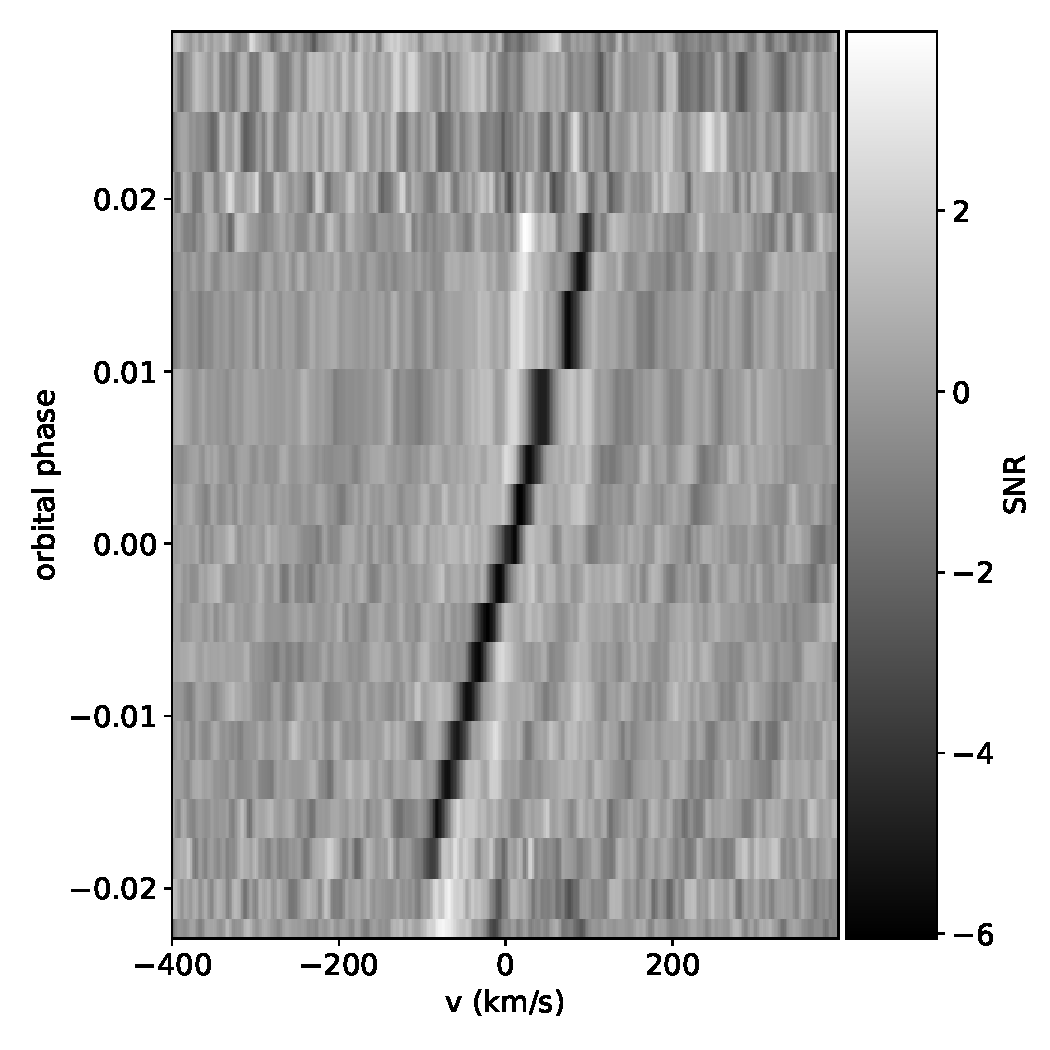
\includegraphics[width=0.25\textwidth]{plots/raw-ccf-before/KELT-20b.20190504.Fe.blue.CCFs-raw.pdf}
                \hspace{0.05\textwidth}
                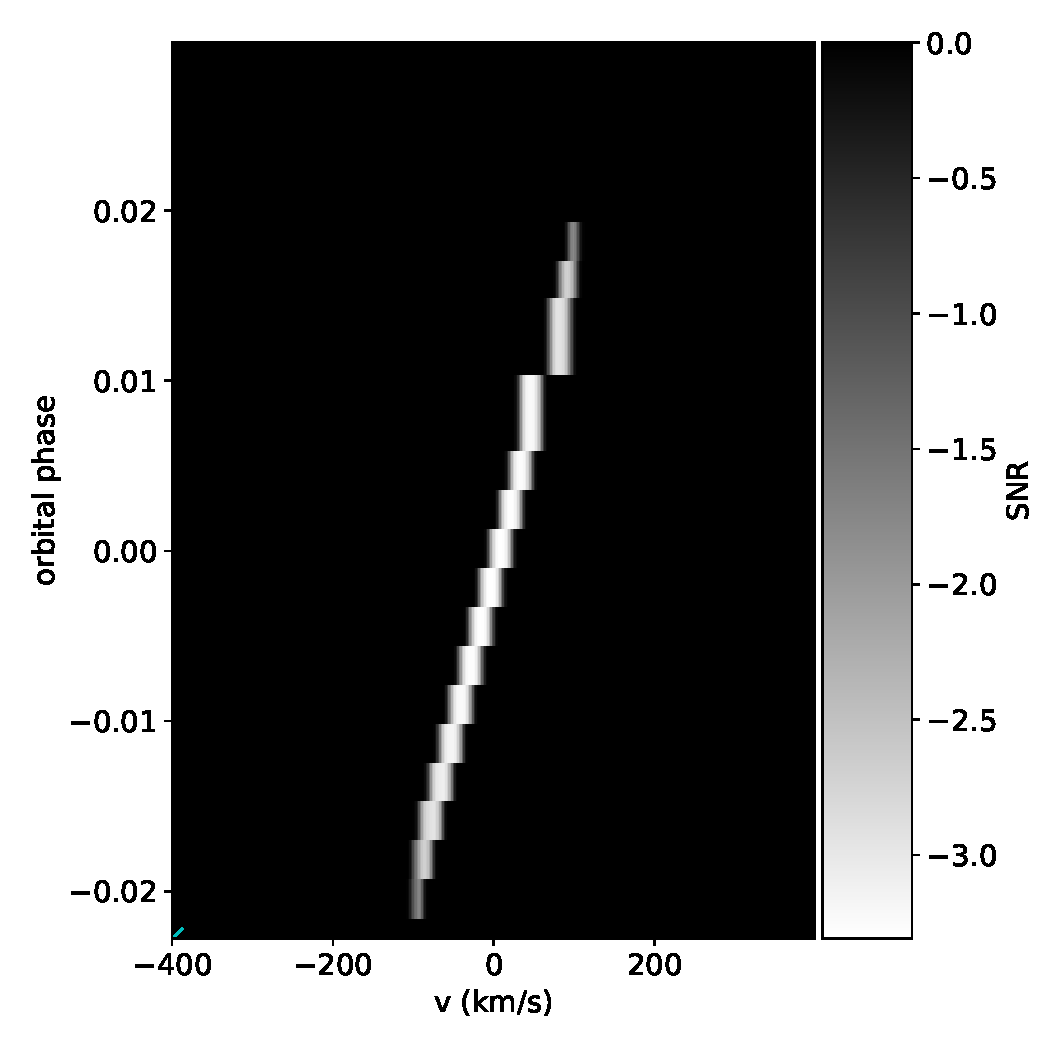
\includegraphics[width=0.25\textwidth]{plots/raw-ccfs/doppler-shadow/KELT-20b.20190504.Fe.blue.DopplerShadow.pdf}
                \hspace{0.05\textwidth}
                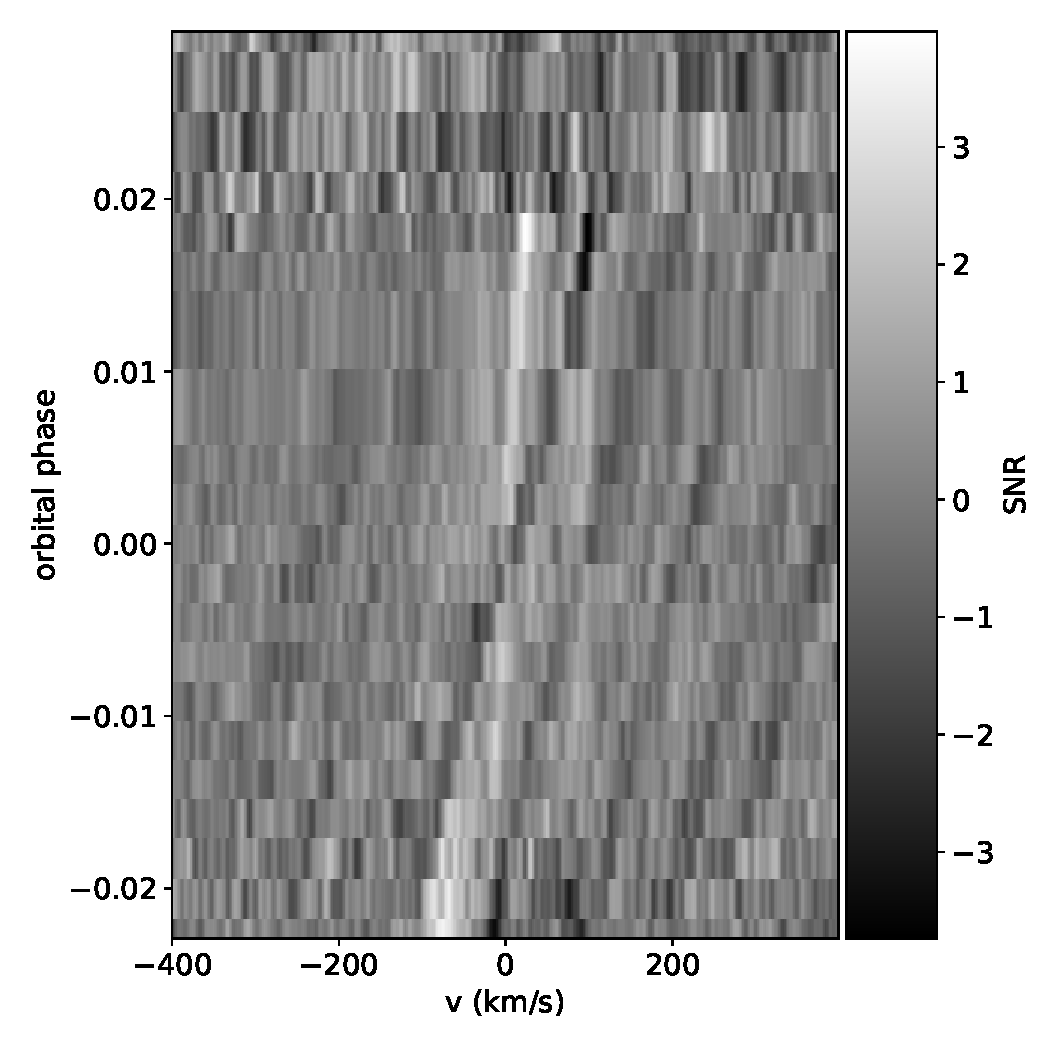
\includegraphics[width=0.25\textwidth]{plots/raw-ccf-after/KELT-20b.20190504.Fe.blue.CCFs-raw.pdf}
                \caption{Removal of the Doppler shadow in the blue arm CCF of Fe I. \textit{Left panel}: CCF of in-transit exposures showing Doppler Shadow (dark streak) intersecting with the radial velocity signal (bright streak). \textit{Right panel}: Residual CCF after subtracting off the Doppler shadow.}
                \label{fig:doppler-shadow-removal}
            \end{figure}
        
        \subsection{Phase-resolved Absorption Signatures}\label{subsec:Line Velocities}

            We repeat the fitting procedure described in Section \ref{subsec:cross-correlation} for each in-transit CCF, in three different phase binning setups. We first examine the ingress-egress line profile asymmetry by binning the CCFs between $T_{12}$ (ingress) and $T_{34}$ (egress) \citep{Lund2017}, selecting the best-fit $K_p$ with a peak center $|\Delta V| \leq 15$ kms$^{-1}$ for each bin. By examining CCFs only during ingress and egress, we can isolate the eastward (trailing) limb and westward (leading) limb flows and specify several asymmetry drivers (See Section \ref{subsec:Atmospheric Dynamics}). Second, we examine the full-transit line profile asymmetry by binning the $T_{1C}$ (first-half) and $T_{C4}$ (second-half) CCFs, again selecting the best-fit $K_p$ with $|\Delta V| \leq 15$ kms$^{-1}$ for each bin. Third, we make three-exposure bins over the course of transit, for a total of seven bins from $T_1$ to $T_4$ (see Table \ref{tab:observation_details}), selecting the expected $K_p$ and holding it constant for all bins (see Table \ref{tab:parameters_summary}). With this binning scheme, we seek to show the behavior of high SNR species during transit with more granularity. We only apply the third phase-binning method to species $\geq4\sigma$ SNR, as tentative species do not maintain a significant signal for full the duration of transit.
            
            For each of these binning procedures, we fit a Gaussian to the binned line profiles and plot the CCF amplitude and $\Delta V$ as a function of phase, observing the change in line velocity between bins (see Figure \ref{fig:phase-binned+RVs-results} and Figure \ref{fig:phase-binned+RVs-results}). We intend to constrain the three-dimensional equilibrium mechanisms driving observed phase asymmetries by connecting our observations to UHJ GCMs \citep{Savel2023}. 
            
            % plot of example telluric corrections by molecfit
            
            % plots showing petitRADTRANS-generated model spectra for each species meeting tentative detection threshold
            
    \section{Results}\label{sec:Results}

        
        \subsection{Detections}\label{subsec:Detections}

            To date, high-resolution cross-correlation transmission spectroscopy (HRCCTS) of KELT-20b has yielded detections of Mg I, Fe I, Fe II, Na I, Cr II, and Ca II \citep{CasasayasBarris2019, Hoeijmakers2020, Nugroho2020, Rainer2021, Langeveld2022, Sicilia2022}, all of which we confirm. Additionally, we present a novel detection of Cu I and tentative detections of Cr I, Co I, Zn I, Ca I, and Ti II (see Table \ref{tab:detection-summary} and Figure \ref{fig:CCFs-appendix} for full set of 2D CCFs and 1D CCF.

            Our reported velocity offsets largely do not agree with the literature. In the cases of Mg I, Fe I, Fe II, Na I, Ba II, and Cu I, we find either a redshifted velocity offset or, given the uncertainty, velocity offsets consistent with zero—none of which match the findings of \citet{CasasayasBarris2019, Stangret2020, Hoeijmakers2020, Nugroho2020, Rainer2021, Langeveld2022, BelloArufe2022}.


            
            \begin{deluxetable*}{lcccccccc}\label{tab:detection-summary}
                \tablecaption{}
                \tablehead{
                    \colhead{} & 
                    \colhead{\textbf{Spectrograph}} & 
                    \colhead{\textbf{Arm}} &
                    \colhead{\textbf{$N_{\text{obs}}$}} &
                    \colhead{\textbf{Species}} & 
                    \colhead{\textbf{SNR ($\sigma$)}} & 
                    \colhead{\textbf{$\Delta V$ ($\text{km}\,\text{s}^{-1}$)}} & 
                    \colhead{\textbf{FWHM ($\text{km}\,\text{s}^{-1}$})} &
                    \colhead{\textbf{$K_p$ ($\text{km}\,\text{s}^{-1}$)}}
                }
                
                \startdata
                    \textbf{This Work} & PEPSI & Blue & 1 & Mg I & $5.43 \pm 0.36$ & $-0.15 \pm 0.64$ & $19.77 \pm 1.50$ & $174$ \\
                    & & Combined & & Fe I & $5.29 \pm 0.65$ & $0.34 \pm 0.51$ & $8.53 \pm 1.20$ & $209$ \\
                    & & Combined & & Fe II & $15.46 \pm 1.04$ & $1.14 \pm 0.22$ & $6.61 \pm 0.51$ & $163$ \\
                    & & Combined & & Na I & $4.43 \pm 0.60$ & $6.59 \pm 0.53$ & $8.01 \pm 1.24$ & $249$ \\
                    & & Red & & Ba II & $3.30 \pm 0.31$ & $0.28 \pm 1.55$ & $33.23 \pm 3.66$ & $268$ \\
                    & & Blue & & Cu I & $3.56 \pm 0.49$ & $2.33 \pm 0.62$ & $9.15 \pm 1.46$ & $220$ \\
                    & & Blue & & Cr I & $4.54 \pm 0.44$ & $-1.14 \pm 0.55$ & $11.61 \pm 1.30$ & $209$ \\
                    & & Blue & & Mn I & $3.00 \pm 0.48$ & $-3.32 \pm 0.83$ & $10.69 \pm 1.95$ & $257$ \\
                    \citet{CasasayasBarris2019} & HARPS-N & --- & 3 & Fe II & --- & $-2.8 \pm 0.8$ & $7.2 \pm 1.2$ & $174.4 \pm 14.0$ \\
                    & & --- & & Na I & --- & $-3.1 \pm 0.9$ & $9.2 \pm 2.0$ & $176.6 \pm 11.7$ \\
                    & & --- & & $H_{\alpha}$ & --- & $-3.0 \pm 1.2$ & $19.0 \pm 1.6$ & $165.6 \pm 16.7$ \\
                    & & --- & & $H_{\beta}$ & --- & $-1.2 \pm 1.4$ & $19.4 \pm 2.5$ & $136.2 \pm 18.6$ \\
                    & & --- & & $H_{\gamma}$ & --- & $-2.3 \pm 2.7$  & $16.6 \pm 4.2$ & $135.0 \pm 34.8$ \\
                    & CARMENES & --- & 1 & Na I & --- & $-3.2 \pm 1.7$ & $8.0 \pm 1.2$ & $182.5 \pm 14.3$ \\
                    & & --- & & Ca II & --- & $-1.9 \pm 0.6$ & $9.2 \pm 1.0$ & $157.7 \pm 8.2$ \\
                    & & --- & & $H_{\alpha}$ & --- & $-4.5 \pm 0.5$ & $22.6 \pm 0.9$ & $166.2 \pm 7.4$ \\
                    \citet{Stangret2020} & HARPS-N & --- & 3 & Fe I & $10.5 \pm 0.4$& $-6.3\pm 0.8$ & --- & $121^{+86}_{-29}$\\
                    & & --- & & Fe II & $8.6 \pm 0.5$  & $-2.8 \pm 0.8$  & --- & $155^{+18}_{-18}$ \\
                    \citet{Hoeijmakers2020} & EXPRES & --- & 1 & Mg I & $3.33$ & $-8.40 \pm 1.40$ & $33.45 \pm 3.30$ & 175 \\
                    & & --- & & Fe I & $3.45$ & $-4.81 \pm 0.72$ & $12.39 \pm 1.69$ & 175 \\
                    & & --- & & Fe II & $4.60$ & $-0.75 \pm 0.37$ & $8.54 \pm 0.87$ & 175 \\
                    & & --- & & Na I & $3.40$ & $-4.38 \pm 0.54$ & $10.07 \pm 1.26$ & 175 \\
                    & & --- & & Cr II & $3.69$ & $-3.40 \pm 0.42$ & $5.31 \pm 0.99$ & 175 \\
                    \citet{Nugroho2020} & HARPS-N & --- & 3 & Fe I & $14.30$ & $-3.6 \pm 0.3$ & & $200.1 \pm 5.2$ \\
                    & & --- & & Fe II & $14.61$ & $-1.4 \pm 0.2$ & & $165.0 \pm 3.5$ \\
                    & & --- & & Na I & $7.72$ & $-1.4 \pm 0.7$ & & $180.0 \pm 11.8$ \\
                    & & --- & & Ca II & $7.53$ & $2.2 \pm 1.2$ & & $138.5 \pm 15.3$\\
                    & CARMENES & --- & 1 & Fe I & $6.44$ & $-6.5 \pm 0.6$ &  & $263.1 \pm 8.8$\\
                    &          & --- &   & Fe II &$3.60$ & $-0.4 \pm 0.6$ &  & $139.2 \pm 2.5$\\
                    &          & --- &   & Na I  &$6.83$ & $-0.6 \pm 0.7$ &  & $167.3 \pm 12.1$\\
                    &          & --- &   & Ca II &$8.60$ & $0.1 \pm 0.6$ &   & $174.8 \pm 8.2$ \\
                    \citet{Kesseli2020} & CARMENES & --- & 1 & FeH & $3.02$ & $-0.5$ &  & $158$ \\
                    \citet{Rainer2021} & HARPS-N & --- & 5 & Fe I & --- & $-4.7^{+0.3}_{-0.7}$ &  & $147^{+7}_{-6}$\\
                    \citet{Langeveld2022} & HARPS-N & --- & 3 & Na I & --- & $-3.1 \pm 1.9$ & --- & \\
                    \citet{Sicilia2022} & HARPS-N & --- & 3 & $H_{\alpha}$ & --- & $-5.2^{+1.8}_{-1.7}$ & $27.9^{+3.7}_{-3.3}$ &$156.3^{+28.5}_{-27.0}$ \\
                    & & --- & & Na I D$_1$ & --- & $-3.8^{+0.7}_{-0.7}$ & $12.5^{+2.9}_{-2.3}$ & $192.5^{+12.4}_{-13.5}$\\
                    & & --- & & Na I D$_2$ & --- & $-3.7^{+0.9}_{-0.9}$ & $14.8^{+2.8}_{-2.4}$ & $170.0^{+14.9}_{-13.5}$\\
                    \citet{BelloArufe2022} & FIES & --- & 2 & Fe II & $5.3$& $-20^{+6}_{-6}$ & --- & $120^{+78}_{-46}$\\
                    \enddata
            \end{deluxetable*}

            \clearpage
            
        \subsection{Atmospheric Dynamics}\label{subsec:Atmospheric Dynamics}

            As KELT-20b begins its transit, we expect that the day-night winds, carrying Fe I and Fe II from the hot dayside to the cool nightside, to be evidenced by blueshifted velocity offsets of these species. However, this is not observed; instead, we observe slightly redshifted velocities in both Fe I and Fe II (See Table \ref{tab:detection-summary}). We present these results as a challenge to the theory of phase-resolved velocities predicted hitherto, compiled in \citet{Savel2023}. We suggest the driver of this asymmetry is a westward hotspot offset which causes the leading limb of the atmosphere to be hotter. As a result, the leading limb's scale height is greater than the trailing limb's, making it more susceptible to be probed by transmission spectroscopy and thereby increasing the first-half 1D CCF amplitude relative to the second-half's.
    
            Fe I ($X\sigma$) and Fe II ($X\sigma$) are our strongest detections, each exhibiting distinct physical behavior shown in Figure \ref{fig:phase-binned-1d-ccfs-Fe/Fe+}. When analyzing their phase-resolved velocity offsets, we observe a quasi-consistent offset between the species, suggesting that Fe I and Fe II are being probed at different atmospheric pressures. A potential driver for this offset is a photoionized layer of Fe II, which is more abundant at lower pressures and more easily probed by transmission spectroscopy. It must be noted that Fe I and Fe II do alias, although when using a full-transit bin as presented in Figure \ref{fig:aliases}, the aliasing peak does not occur at the 
            
            The differential rotation of the atmosphere, with a faster-moving upper layer primarily composed of Fe II, should cause the magnitude of Fe II's velocity offset, $|\Delta V|$, to consistently exceed Fe I's during transit. This interpretation is supported by the observed discrepancy in the FWHM between the species (see Table \ref{tab:detection-summary}) attributed to pressure broadening of the Fe I lines. Another factor to consider is the scale height effect \citep{Savel2023}. 
            
            The hotter leadeing limb of the planet has a larger scale height, making it more amenable to be probed by transmission spectroscopy \citep{Prinoth2023}. This is supported by the 1D CCF phase asymmetries observed when binning the data into half-phase and ingress/egress bins. We consistently observe higher CCF amplitudes in the first half and ingress bins compared to the second half and egress bins.

            

        \begin{figure*} \label{fig:phase-binned-1d-ccfs-Fe/Fe+}
            \centering
            \gridline{
                \fig{plots/line-profile-phasebinned/ingress-egress/blue/KELT-20b.20190504.blue.Fe..ingress-egress.SNR-Gaussian-Asymmetry.pdf}{0.33\textwidth}{}
                \fig{plots/line-profile-phasebinned/halves/blue/KELT-20b.20190504.blue.Fe..halves.SNR-Gaussian-Asymmetry.pdf}{0.33\textwidth}{}
                \fig{plots/line-profile-phasebinned/3-exposure/blue/KELT-20b.Fe.blue.phase-binned+RVs.pdf}{0.33\textwidth}{}
            }
            \gridline{
                \fig{plots/line-profile-phasebinned/ingress-egress/blue/KELT-20b.20190504.blue.Fe+..ingress-egress.SNR-Gaussian-Asymmetry.pdf}{0.33\textwidth}{}
                \fig{plots/line-profile-phasebinned/halves/blue/KELT-20b.20190504.blue.Fe+..halves.SNR-Gaussian-Asymmetry.pdf}{0.33\textwidth}{}
                \fig{plots/line-profile-phasebinned/3-exposure/blue/KELT-20b.Fe+.blue.phase-binned+RVs.pdf}{0.33\textwidth}{}
            }
            \caption{\textit{Top:} Line profile dynamics of Fe I as observed by PEPSI's blue arm. From left to right: ingress and egress phase-binned 1D CCF, first half and second half of transit phase-binned 1D CCF, center of Gaussian fit to the 1D CCF phase-binned line profile with SNR coloring; three exposures are binned together, making 7 bins from 21 total exposures. \textit{Bottom:} The same plots for Fe II.}
        \end{figure*}

        \ref{fig:phase-binned-1d-ccfs-Fe/Fe+}

                    
        \subsection{Nondetections}\label{subsec:Nondetections}
        
            We do not reproduce detections of H I, Ca II, Cr II, and FeH 
        
            \citep{CasasayasBarris2019, Nugroho2020, Hoeijmakers2020, Kesseli2020}. See Figure \ref{fig:nondetections}. We rule out aliasing causing any spurious detections. For 1D and 2D aliased CCFs of each search species with the Fe I and Fe II templates, see Figure \ref{fig:aliases}.

    \section{Conclusions}\label{sec:Conclusions}


    \vspace{5mm}
    \facilities{LBT}

    \software{astropy \citep{astropy}, 
            Jupyter \citep{jupyter},
            matplotlib \citep{Matplotlib},
            molecfit \citep{Kausch2015, Smette2015},
            numpy \citep{NumPy},
            petitRADTRANS \citep{petitRADTRANS},
            PyFastChem \citep{PyFastChem},
            uncertainties~\citet{uncertainties}
            }

    %% Appendix material should be preceded with a single \appendix command.
    %% There should be a \section command for each appendix. Mark appendix
    %% subsections with the same markup you use in the main body of the paper.

    %% Each Appendix (indicated with \section) will be lettered A, B, C, etc.
    %% The equation counter will reset when it encounters the \appendix
    %% command and will number appendix equations (A1), (A2), etc. The
    %% Figure and Table counter will not reset.

\appendix  

    \section{Model transmission spectra}\label{app:Model transmission spectra}
    \begin{figure}
        \label{fig:model-spectra-appendix}
        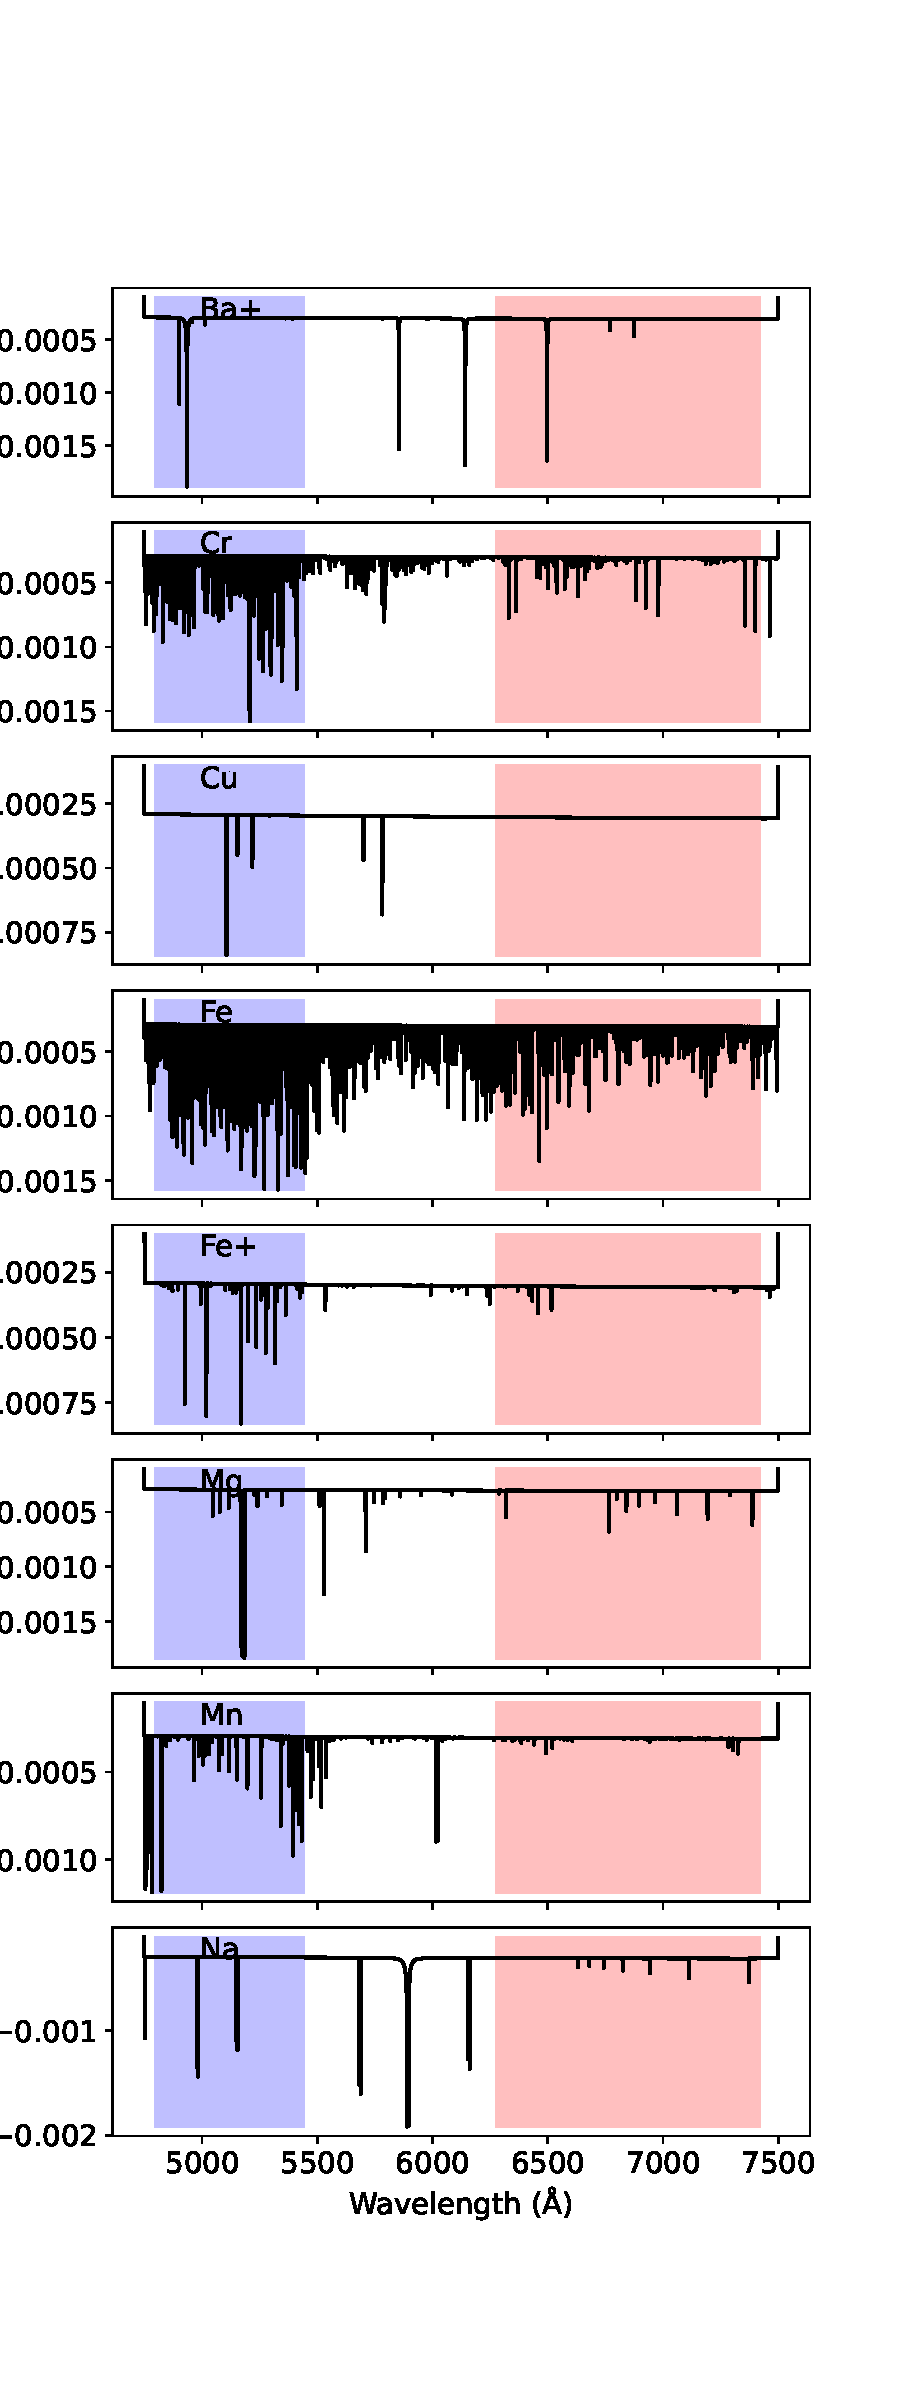
\includegraphics[width=0.33\textwidth]{plots/spectra/spectra.KELT-20b.inverted-transmission-better.pdf}
        % Add additional subfigures as needed
    \caption{Model transmission spectra generated by \code{petitRADTRANS}, with the wavelength coverage of CD III and CD V shown in red and blue respectively.}
            
        \end{figure}    


   \section{Detections}\label{app:Detections}

        \begin{figure}
            \label{fig:CCFs-appendix}
            \centering
            \gridline{
                \fig{plots/line-profile-overlaidarms/KELT-20b.20190504.combined.Mg I.line-profiles-overlaidarms.pdf}{0.25\textwidth}{}
                \fig{plots/raw-ccfs/blue/KELT-20b.20190504.False.Mg.blue.CCFs-raw.pdf}{0.25\textwidth}{\label{fig:raw-ccf-Mg-blue}}
                \fig{plots/kp-vsys-map/blue/KELT-20b.20190504.blue.Mg.CCFs-shifted.pdf}{0.25\textwidth}{\label{fig:2d-ccf-Mg-blue}}
                \fig{plots/line-profile/blue/KELT-20b.20190504.blue.Mg.SNR-Gaussian.pdf}{0.25\textwidth}{\label{fig:1d-ccf-Mg-blue}}
            }
            \gridline{
                \fig{plots/line-profile-overlaidarms/KELT-20b.20190504.combined.Fe I.line-profiles-overlaidarms.pdf}{0.25\textwidth}{}
                \fig{plots/raw-ccfs/combined/KELT-20b.combined.False.Fe..CCFs-raw.pdf}{0.25\textwidth}{\label{fig:raw-ccf-Fe-blue}}
                \fig{plots/kp-vsys-map/combined/KELT-20b.20190504.combined.Fe.CCFs-shifted.pdf}{0.25\textwidth}{\label{fig:2d-ccf-Fe-combined}}
                \fig{plots/line-profile/combined/KELT-20b.20190504.combined.Fe.SNR-Gaussian.pdf}{0.25\textwidth}{\label{fig:1d-ccf-Fe-combined}}
            }
            \gridline{
                \fig{plots/line-profile-overlaidarms/KELT-20b.20190504.combined.Fe II.line-profiles-overlaidarms.pdf}{0.25\textwidth}{}
                \fig{plots/raw-ccfs/combined/KELT-20b.combined.False.Fe+..CCFs-raw.pdf}{0.25\textwidth}{\label{fig:raw-ccf-FeII-combined}}
                \fig{plots/kp-vsys-map/combined/KELT-20b.20190504.combined.Fe+.CCFs-shifted.pdf}{0.25\textwidth}{\label{fig:2d-ccf-FeII-combined}}
                \fig{plots/line-profile/combined/KELT-20b.20190504.combined.Fe+.SNR-Gaussian.pdf}{0.25\textwidth}{\label{fig:1d-ccf-FeII-combined}}
            }
            \gridline{
                \fig{plots/line-profile-overlaidarms/KELT-20b.20190504.combined.Na I.line-profiles-overlaidarms.pdf}{0.25\textwidth}{}
                \fig{plots/raw-ccfs/red/KELT-20b.20190504.False.Na.red.CCFs-raw.pdf}{0.25\textwidth}{\label{fig:raw-ccf-Na-combined}}
                \fig{plots/kp-vsys-map/red/KELT-20b.20190504.red.Na.CCFs-shifted.pdf}{0.25\textwidth}{\label{fig:2d-ccf-Na-combined}}
                \fig{plots/line-profile/red/KELT-20b.20190504.red.Na.SNR-Gaussian.pdf}{0.25\textwidth}{\label{fig:1d-ccf-Na-combined}}
            }
        \end{figure}

        \begin{figure}
            \gridline{
                \fig{plots/line-profile-overlaidarms/KELT-20b.20190504.combined.Ba II.line-profiles-overlaidarms.pdf}{0.25\textwidth}{}
                \fig{plots/raw-ccfs/red/KELT-20b.20190504.Ba+.red.CCFs-raw.pdf}{0.25\textwidth}{\label{fig:raw-ccf-Ba-blue}}
                \fig{plots/kp-vsys-map/red/KELT-20b.20190504.red.Ba+.CCFs-shifted.pdf}{0.25\textwidth}{\label{fig:2d-ccf-Ba+-blue}}
                \fig{plots/line-profile/red/KELT-20b.20190504.red.Ba+.SNR-Gaussian.pdf}{0.25\textwidth}{\label{fig:1d-ccf-Ba+-blue}}
            }
            \gridline{
                \fig{plots/line-profile-overlaidarms/KELT-20b.20190504.combined.Cu I.line-profiles-overlaidarms.pdf}{0.25\textwidth}{}
                \fig{plots/raw-ccfs/blue/KELT-20b.20190504.Cu.blue.CCFs-raw.pdf}{0.25\textwidth}{\label{fig:raw-ccf-Cu-blue}}
                \fig{plots/kp-vsys-map/blue/KELT-20b.20190504.blue.Cu.CCFs-shifted.pdf}{0.25\textwidth}{\label{fig:2d-ccf-Cu-blue}}
                \fig{plots/line-profile/blue/KELT-20b.20190504.blue.Cu.SNR-Gaussian.pdf}{0.25\textwidth}{\label{fig:1d-ccf-Cu-blue}}
            }

            \gridline{
                \fig{plots/line-profile-overlaidarms/KELT-20b.20190504.combined.Mn I.line-profiles-overlaidarms.pdf}{0.25\textwidth}{}
                \fig{plots/raw-ccfs/blue/KELT-20b.20190504.False.Mn.blue.CCFs-raw.pdf}{0.25\textwidth}{\label{fig:raw-ccf-Mn-blue}}
                \fig{plots/kp-vsys-map/blue/KELT-20b.20190504.blue.Mn.CCFs-shifted.pdf}{0.25\textwidth}{\label{fig:2d-ccf-Mn-blue}}
                \fig{plots/line-profile/blue/KELT-20b.20190504.blue.Mn.SNR-Gaussian.pdf}{0.25\textwidth}{\label{fig:1d-ccf-Mn-blue}}
            }
            
            \caption{Cross-correlation results for each detected and tentatively detected atomic species in our analysis. \textit{Left panel}: $K_p-RV$ maps in the stellar rest frame. \textit{Middle panel}: $K_p-\Delta V$ maps, shifted into the planetary rest frame. \textit{Right panel}: $SNR-\Delta V$ map at the $K_p$ corresponding to peak signal. This figure shows the maps, 1D CCFs, and line profiles for each species exceeding the ${3\sigma}$ tentative detection threshold. The offset of the center of the 1D CCF Gaussian from the planetary rest frame, $\Delta V$, denotes the line velocity.}
        \end{figure}
        
    \section{Dynamics}\label{app:Dynamics}
    
        \begin{figure}
            \centering
            \gridline{
                \fig{plots/line-profile-phasebinned/ingress-egress/blue/KELT-20b.20190504.blue.Mg..ingress-egress.SNR-Gaussian-Asymmetry.pdf}{0.33\textwidth}{}
                \fig{plots/line-profile-phasebinned/halves/blue/KELT-20b.20190504.blue.Mg..halves.SNR-Gaussian-Asymmetry.pdf}{0.33\textwidth}{}
                \fig{plots/line-profile-phasebinned/3-exposure/blue/KELT-20b.Mg.blue.phase-binned+RVs.pdf}{0.33\textwidth}{}
            }
            \gridline{
                \fig{plots/line-profile-phasebinned/ingress-egress/blue/KELT-20b.20190504.blue.Fe..ingress-egress.SNR-Gaussian-Asymmetry.pdf}{0.33\textwidth}{}
                \fig{plots/line-profile-phasebinned/halves/blue/KELT-20b.20190504.blue.Fe..halves.SNR-Gaussian-Asymmetry.pdf}{0.33\textwidth}{}
                \fig{plots/line-profile-phasebinned/3-exposure/blue/KELT-20b.Fe.blue.phase-binned+RVs.pdf}{0.33\textwidth}{}
            }
            \gridline{
                \fig{plots/line-profile-phasebinned/ingress-egress/blue/KELT-20b.20190504.blue.Fe+..ingress-egress.SNR-Gaussian-Asymmetry.pdf}{0.33\textwidth}{}
                \fig{plots/line-profile-phasebinned/halves/blue/KELT-20b.20190504.blue.Fe+..halves.SNR-Gaussian-Asymmetry.pdf}{0.33\textwidth}{}
                \fig{plots/line-profile-phasebinned/3-exposure/blue/KELT-20b.Fe+.blue.phase-binned+RVs.pdf}{0.33\textwidth}{}
            }
            \gridline{
                \fig{plots/line-profile-phasebinned/ingress-egress/blue/KELT-20b.20190504.blue.Na..ingress-egress.SNR-Gaussian-Asymmetry.pdf}{0.33\textwidth}{}
                \fig{plots/line-profile-phasebinned/halves/blue/KELT-20b.20190504.blue.Na..halves.SNR-Gaussian-Asymmetry.pdf}{0.33\textwidth}{}
                \fig{plots/line-profile-phasebinned/3-exposure/blue/KELT-20b.Na.blue.phase-binned+RVs.pdf}{0.33\textwidth}{}
            }

        \end{figure}


        \begin{figure}
            \gridline{
                \fig{plots/line-profile-phasebinned/ingress-egress/red/KELT-20b.20190504.red.Ba+..ingress-egress.SNR-Gaussian-Asymmetry.pdf}{0.33\textwidth}{}
                \fig{plots/line-profile-phasebinned/halves/red/KELT-20b.20190504.red.Ba+..halves.SNR-Gaussian-Asymmetry.pdf}{0.33\textwidth}{}
                \fig{plots/line-profile-phasebinned/3-exposure/red/KELT-20b.Ba+.red.phase-binned+RVs.pdf}{0.33\textwidth}{}
            }
            \gridline{
                \fig{plots/line-profile-phasebinned/ingress-egress/blue/KELT-20b.20190504.blue.Cu..ingress-egress.SNR-Gaussian-Asymmetry.pdf}{0.33\textwidth}{}
                \fig{plots/line-profile-phasebinned/halves/blue/KELT-20b.20190504.blue.Cu..halves.SNR-Gaussian-Asymmetry.pdf}{0.33\textwidth}{}
                \fig{plots/line-profile-phasebinned/3-exposure/blue/KELT-20b.Cu.blue.phase-binned+RVs.pdf}{0.33\textwidth}{}
            }
            \gridline{
                \fig{plots/line-profile-phasebinned/ingress-egress/blue/KELT-20b.20190504.blue.Cr..ingress-egress.SNR-Gaussian-Asymmetry.pdf}{0.33\textwidth}{}
                \fig{plots/line-profile-phasebinned/halves/blue/KELT-20b.20190504.blue.Cr..halves.SNR-Gaussian-Asymmetry.pdf}{0.33\textwidth}{}
                \fig{plots/line-profile-phasebinned/3-exposure/blue/KELT-20b.Cr.blue.phase-binned+RVs.pdf}{0.33\textwidth}{}
            }
            \gridline{
                \fig{plots/line-profile-phasebinned/ingress-egress/blue/KELT-20b.20190504.blue.Mn..ingress-egress.SNR-Gaussian-Asymmetry.pdf}{0.33\textwidth}{}
                \fig{plots/line-profile-phasebinned/halves/blue/KELT-20b.20190504.blue.Mn..halves.SNR-Gaussian-Asymmetry.pdf}{0.33\textwidth}{}
                \fig{plots/line-profile-phasebinned/3-exposure/blue/KELT-20b.Mn.blue.phase-binned+RVs.pdf}{0.33\textwidth}{}
            }
            \caption{Phase-binned radial velocity measurements}
            \label{fig:phase-binned+RVs-results}
        \end{figure}
        
        \begin{figure}[]\label{fig:combined-line-profiles-appendix} 
            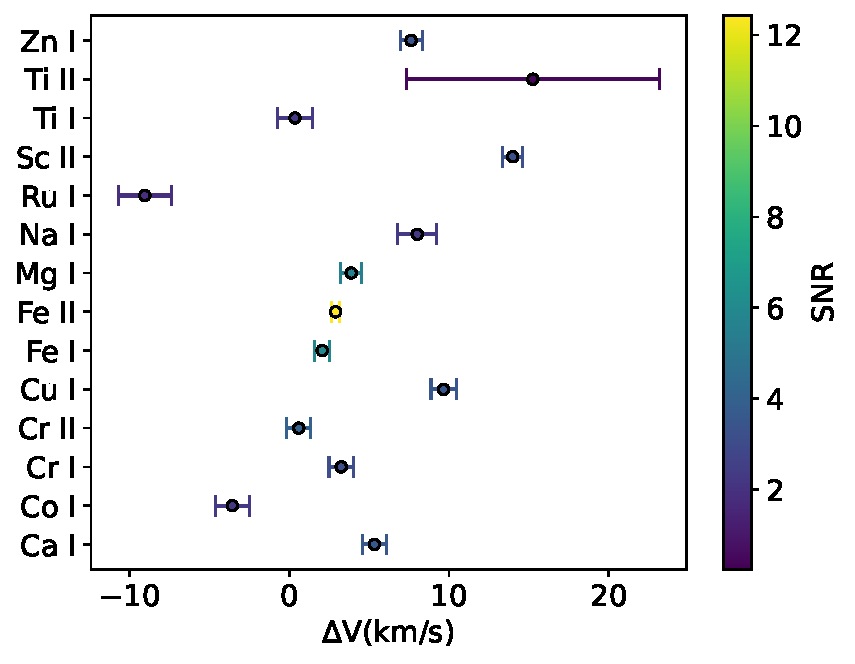
\includegraphics[width=0.45\textwidth]{plots/KELT-20b.inverted-transmission-better.CombinedRVs.pdf}
            \caption{The net Doppler shifts of each detected species, ordered and colored by their peak detection SNR.}
            
        \end{figure}



    \section{Nondetections}\label{app:Nondetections}
        \begin{figure}
        \centering
            \gridline{
                \fig{plots/raw-ccfs/blue/KELT-20b.20190504.Ca+.blue.CCFs-raw.pdf}{0.25\textwidth}{\label{fig:raw-ccf-Ca+-blue}}
                \fig{plots/kp-vsys-map/blue/KELT-20b.20190504.blue.Ca+.CCFs-shifted.pdf}{0.25\textwidth}{\label{fig:2d-ccf-Ca+-blue}}
                \fig{plots/line-profile/blue/KELT-20b.20190504.blue.Ca+.SNR-Gaussian.pdf}{0.25\textwidth}{\label{fig:1d-ccf-Ca+-blue}}
            }
            \gridline{
                \fig{plots/raw-ccfs/blue/KELT-20b.20190504.Ru.blue.CCFs-raw.pdf}{0.25\textwidth}{\label{fig:raw-ccf-Mg-blue}}
                \fig{plots/kp-vsys-map/blue/KELT-20b.20190504.blue.Ru.CCFs-shifted.pdf}{0.25\textwidth}{\label{fig:2d-ccf-Fe+-blue}}
                \fig{plots/line-profile/blue/KELT-20b.20190504.blue.Ru.SNR-Gaussian.pdf}{0.25\textwidth}{\label{fig:1d-ccf-Fe+-blue}}
            }
            \gridline{
                \fig{plots/raw-ccfs/blue/KELT-20b.20190504.Ti.blue.CCFs-raw.pdf}{0.25\textwidth}{\label{fig:raw-ccf-Mg-blue}}
                \fig{plots/kp-vsys-map/blue/KELT-20b.20190504.blue.Ti.CCFs-shifted.pdf}{0.25\textwidth}{\label{fig:2d-ccf-Fe+-blue}}
                \fig{plots/line-profile/blue/KELT-20b.20190504.blue.Ti.SNR-Gaussian.pdf}{0.25\textwidth}{\label{fig:1d-ccf-Fe+-blue}}
            }
            \gridline{
                \fig{plots/raw-ccfs/blue/KELT-20b.20190504.Sc+.blue.CCFs-raw.pdf}{0.25\textwidth}{\label{fig:raw-ccf-Mg-blue}}
                \fig{plots/kp-vsys-map/blue/KELT-20b.20190504.blue.Sc+.CCFs-shifted.pdf}{0.25\textwidth}{\label{fig:2d-ccf-Fe+-blue}}
                \fig{plots/line-profile/blue/KELT-20b.20190504.blue.Sc+.SNR-Gaussian.pdf}{0.25\textwidth}{\label{fig:1d-ccf-Fe+-blue}}
            }
            
            \label{fig:nondetections}
        \end{figure}


    \section{Aliases}\label{app:Aliases}
        \begin{figure}
            \gridline{
                \fig{plots//aliases//Fe//blue//2d-ccf/KELT-20b.mock-obs.blue.FeMg_Aliasalias.CCFs-shifted.pdf}{0.25\textwidth}{}
                \fig{plots//aliases//Fe//blue//1d-ccf/KELT-20b.mock-obs.blue.FeMg_Aliasalias.SNR-Gaussian.pdf}{0.2\textwidth}{}
                \fig{plots//aliases//Fe+//blue//2d-ccf/KELT-20b.mock-obs.blue.Fe+Mg_Aliasalias.CCFs-shifted.pdf}{0.25\textwidth}{}
                \fig{plots//aliases//Fe+//blue//1d-ccf/KELT-20b.mock-obs.blue.Fe+Mg_Aliasalias.SNR-Gaussian.pdf}{0.2\textwidth}{}
            }
            
            \gridline{
                \fig{plots//aliases//Fe//blue//2d-ccf/KELT-20b.mock-obs.blue.FeFe+_Aliasalias.CCFs-shifted.pdf}{0.25\textwidth}{}
                \fig{plots//aliases//Fe//blue//1d-ccf/KELT-20b.mock-obs.blue.FeFe+_Aliasalias.SNR-Gaussian.pdf}{0.25\textwidth}{}
                \fig{plots//aliases//Fe+//blue//2d-ccf/KELT-20b.mock-obs.blue.Fe+Fe_Aliasalias.CCFs-shifted.pdf}{0.25\textwidth}{}
                \fig{plots//aliases//Fe+//blue//1d-ccf/KELT-20b.mock-obs.blue.Fe+Fe_Aliasalias.SNR-Gaussian.pdf}{0.25\textwidth}{}
            }
            
            \gridline{
                \fig{plots//aliases//Fe//blue/2d-ccf/KELT-20b.mock-obs.blue.FeNa_Aliasalias.CCFs-shifted.pdf}{0.25\textwidth}{}
                \fig{plots//aliases//Fe//blue/1d-ccf/KELT-20b.mock-obs.blue.FeNa_Aliasalias.SNR-Gaussian.pdf}{0.25\textwidth}{}
                \fig{plots//aliases//Fe+//blue/2d-ccf/KELT-20b.mock-obs.blue.Fe+Na_Aliasalias.CCFs-shifted.pdf}{0.25\textwidth}{}
                \fig{plots//aliases//Fe+//blue/1d-ccf/KELT-20b.mock-obs.blue.Fe+Na_Aliasalias.SNR-Gaussian.pdf}{0.25\textwidth}{}
            }
            
            \gridline{
                \fig{plots//aliases//Fe//blue/2d-ccf/KELT-20b.mock-obs.blue.FeMn_Aliasalias.CCFs-shifted.pdf}{0.25\textwidth}{}
                \fig{plots//aliases//Fe//blue/1d-ccf/KELT-20b.mock-obs.blue.FeMn_Aliasalias.SNR-Gaussian.pdf}{0.25\textwidth}{}
                \fig{plots//aliases//Fe+//blue/2d-ccf/KELT-20b.mock-obs.blue.Fe+Mn_Aliasalias.CCFs-shifted.pdf}{0.25\textwidth}{}
                \fig{plots//aliases//Fe+//blue/1d-ccf/KELT-20b.mock-obs.blue.Fe+Mn_Aliasalias.SNR-Gaussian.pdf}{0.25\textwidth}{}
            }
            
            
           
        \end{figure}
        
        \begin{figure}
            \gridline{
                \fig{plots//aliases//Fe//blue/2d-ccf/KELT-20b.mock-obs.blue.FeCr_Aliasalias.CCFs-shifted.pdf}{0.25\textwidth}{}
                \fig{plots//aliases//Fe//blue/1d-ccf/KELT-20b.mock-obs.blue.FeCr_Aliasalias.SNR-Gaussian.pdf}{0.25\textwidth}{}
                \fig{plots//aliases//Fe+//blue/2d-ccf/KELT-20b.mock-obs.blue.Fe+Cr_Aliasalias.CCFs-shifted.pdf}{0.25\textwidth}{}
                \fig{plots//aliases//Fe+//blue/1d-ccf/KELT-20b.mock-obs.blue.Fe+Cr_Aliasalias.SNR-Gaussian.pdf}{0.25\textwidth}{}
                }
            \caption{\textit{First and second from the left:} Aliasing results of each detected species against the Fe I template. \textit{Third and fourth from the left:} Aliasing results of each detected species against the Fe II template.}
            \label{fig:aliases}
        \end{figure}

\clearpage
\bibliography{bibliography}{}
\bibliographystyle{aasjournal}       

\end{document}